\section{Introduction}

The real-world objects that we interact with in our every-day life can be categorized into many thousands and maybe millions of categories. And even a single object can be member of many categories, i.e.\ at different taxonomical levels or in different parts of a taxonomy. For instance, both objects in Figure \ref{fig:cake} are at once instances of \cat{cake}, \cat{cheesecake}, \cat{dessert}, \cat{sweet}, \cat{pastry}, \cat{food} etc. Hence, when speaker name objects, e.g.\ when referring to it, they have to select a lexical item from a complex network of concepts and competing lexical alternatives.

\begin{figure}[htbp]
\begin{center}
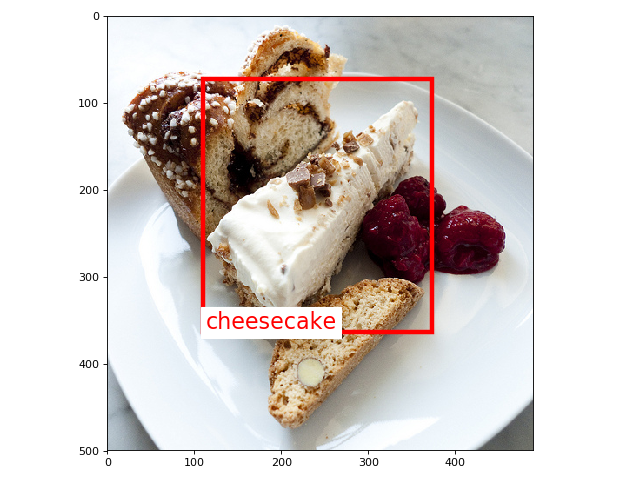
\includegraphics[height=3cm]{Figures/cheescake.png}
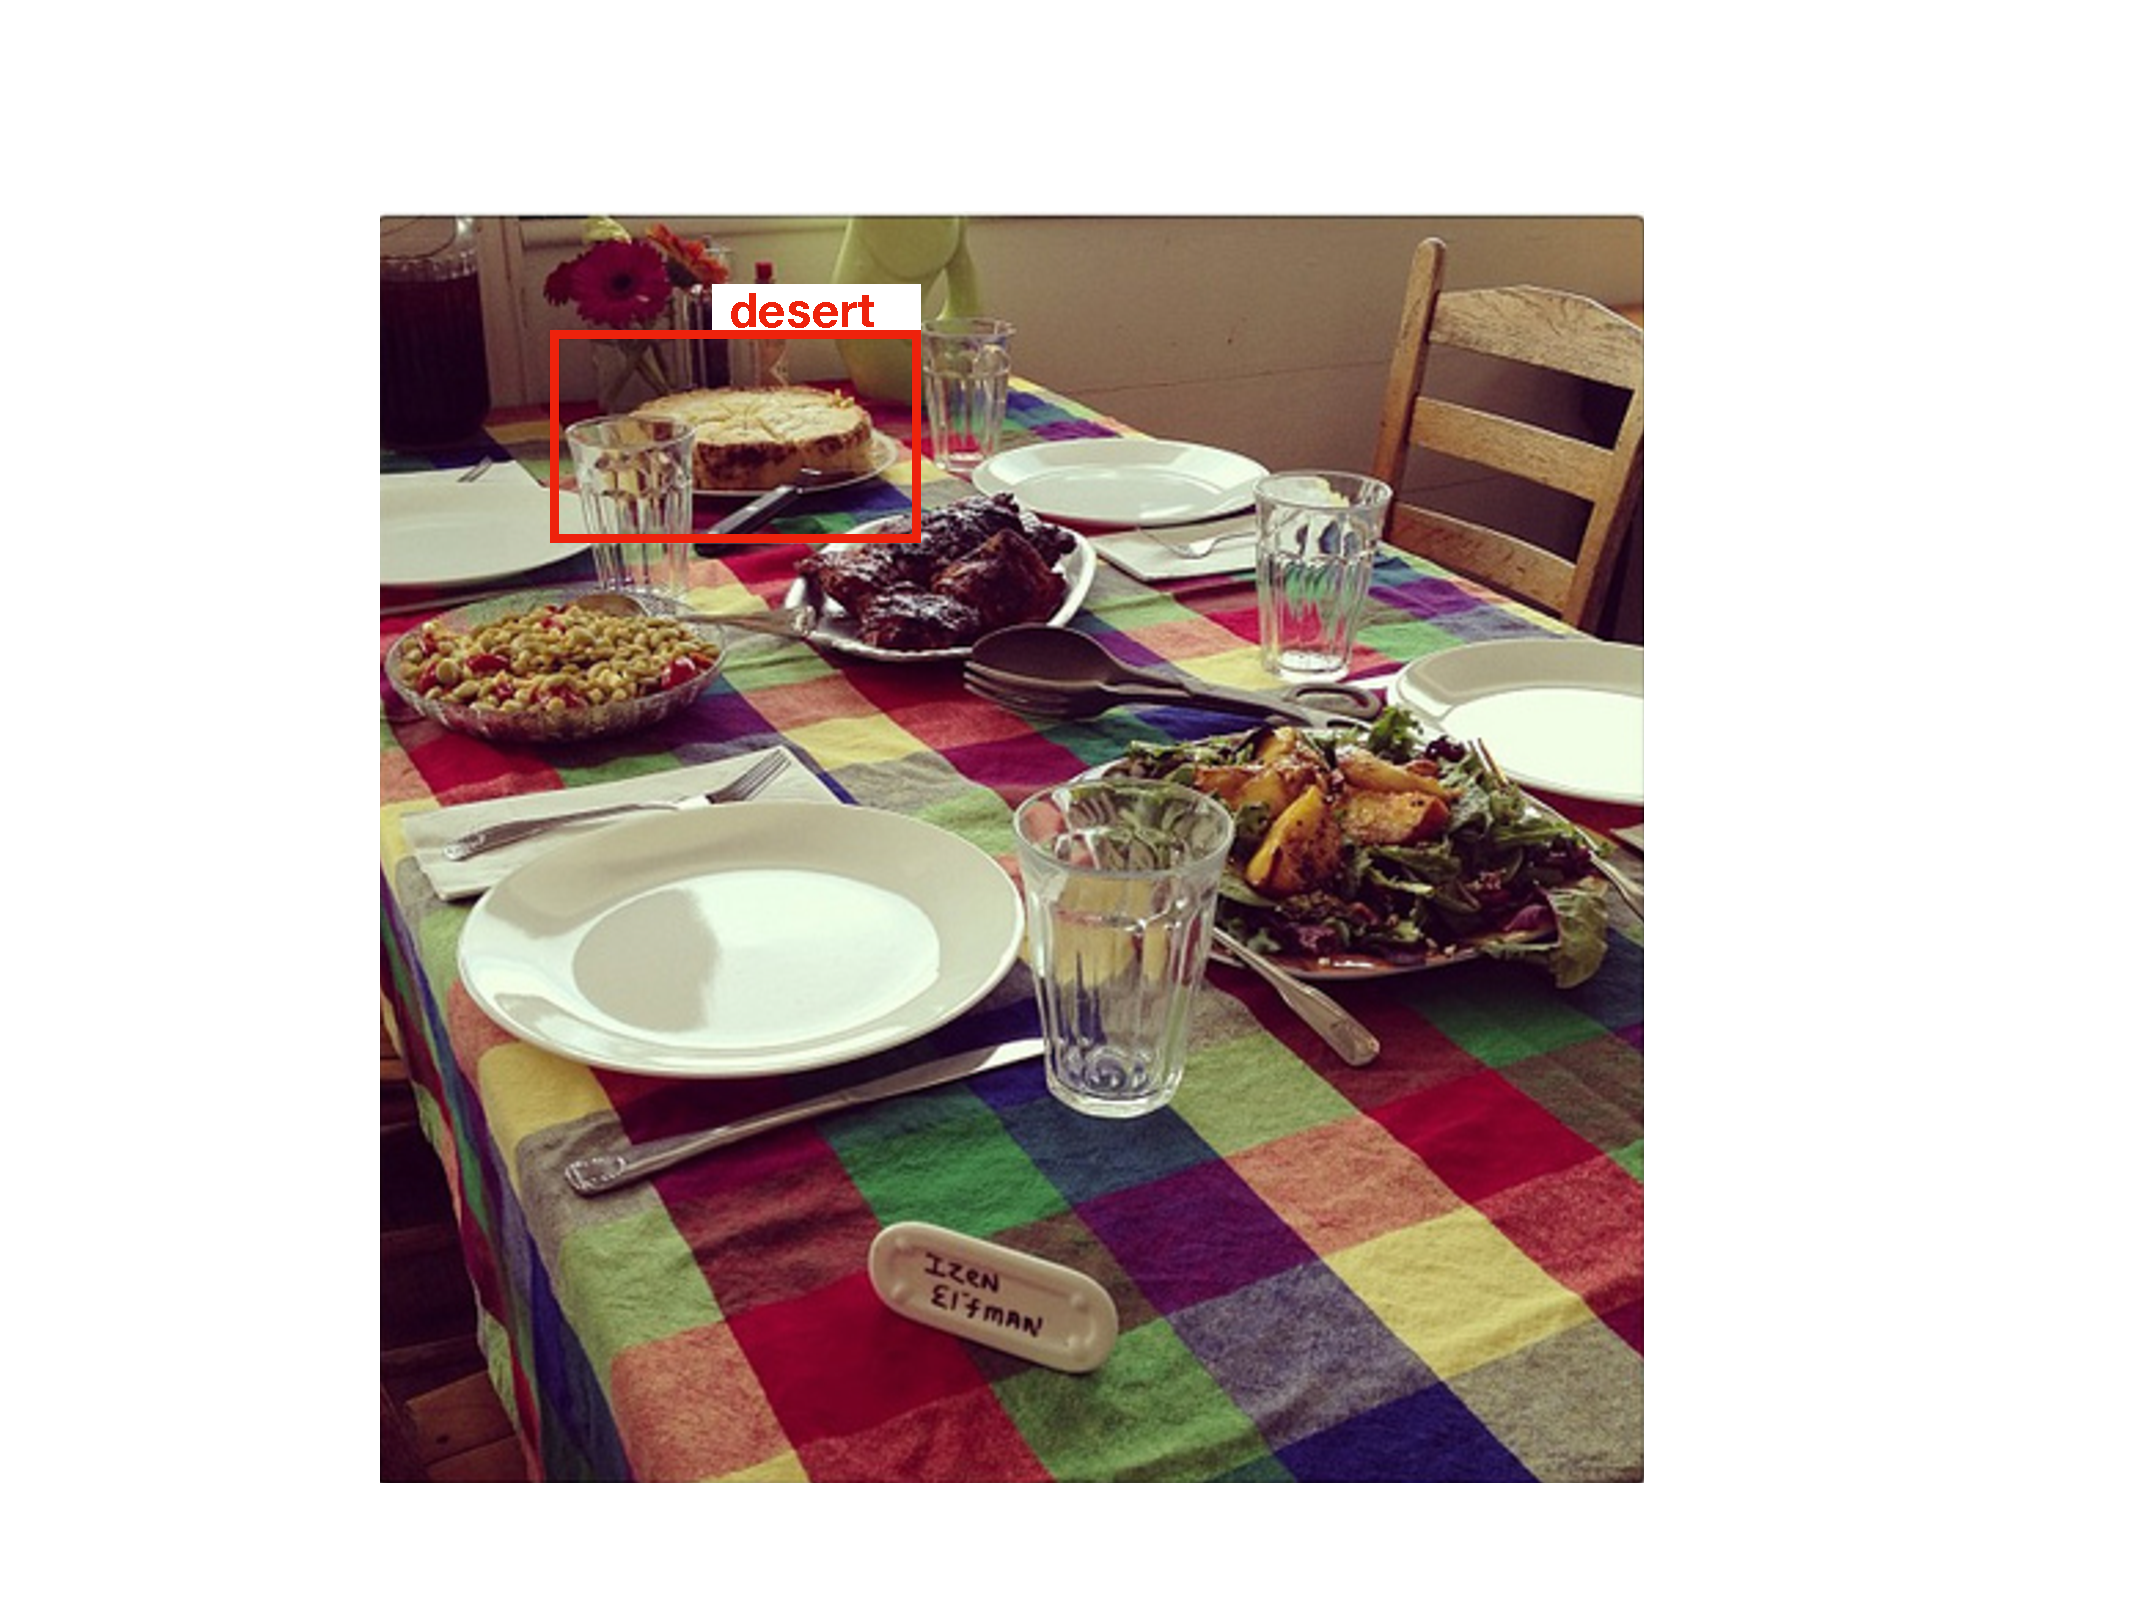
\includegraphics[height=3cm]{Figures/cheesecak2.pdf}
\caption{Two objects of the same type of cake, with different names in VisualGenome}
\label{fig:cake}
\end{center}
\end{figure}


Given the abundance of concepts available in language, the act of \textit{naming} a visual object is not just a labeling of visible properties, it amounts to selecting a name from a complex network of concepts and competing lexical alternatives.
Hence, research on cognition and language production has relied on object naming as a basic paradigm for investigating the processes that underly formation and organization of concepts in the human mind  \cite{rosch1976basic} \sz{cite more here}, though mostly using idealized, graphical objects from specific domains (plants, animals) as visual stimuli.
Complementary to that, research in computer vision has (successfully) focused on automatically recognizing \textit{real-world} objects in images or videos, but using simplified categorization schemes where each object is assigned a single correct label or name, cf.\ \cite{googlenet}. %Here, powerful models have been developed recently that classify visual objects in real-world images into thousands of different (mutually exclusive) categories \newcite{googlenet}.

In NLP, to date, research on object naming is relatively scarce despite the fact that
 there has been a recent explosion of interest in various, and even complex, language \& vision tasks ranging from image captioning \cite{fangetal:2015,devlin:imcaqui,Bernardietal:automatic} to e.g.\ visual dialogue \cite{das2017visual,vries2017guesswhat}. Massive data collections for applications in language \& vision (L\&V) are nowadays available and, in principle, these should also constitute an excellent, large-scale test bed for assessing  theories such as, e.g.\ , the claim that objects have a preferred entry-level when being named  \cite{rosch1976basic}.
%In this paper, we argue that a lot of research in this area would benefit from a deeper and more systematic understanding of the semantic and taxonomic processes in object naming, which is a core phenomenon in virtually every vision \& language task.
%At the same time, we argue that existing resources in L\&V constitute an excellent, large-scale test bed for assessing traditional claims and theories such as, e.g.\ the existence of so-called entry-level categories  \cite{rosch1976basic}.

The goal of this paper is to extend Visual Genome  \cite{krishna2016visualgenome}, a well-known, large-scale resource in language \& vision research, in a way that it can serve as a broad empirical basis for systematic and linguistically motivated investigations into object naming. 
We argue that object naming is an interesting, core phenomenon in itself as it occurs in virtually every L\&V task, but our approach can also support more systematic analysis of broader tasks, such as e.g.\ modeling referring expressions.

Even though VisualGenome is one of the most exhaustively annotated resources to date, providing dense object annotations and descriptions in real-world images, it suffers from two important shortcomings if one is interested in linguistic analysis of object naming:  
First, it only provides a single, manually annotated object description (including a single name) per object which makes it impossible to assess how representative the annotated naming choices are, e.g.\ whether speakers tend to generally prefer \refexp{cheesecake} for the highlighted object in Figure \ref{fig:cake}.
Second, it does not provide consistent taxonomic information on objects and their categories, as names have been automatically linked to WordNet synsets. 
This makes it difficult to assess how naming depends on the taxonomic properties of the object, e.g.\  that both objects in Figure \ref{fig:cake} are instances of \cat{cheesecake}, but one is named \refexp{cheesecake} and the other one is named \refexp{desert}. It is important to note here that these shortcomings exist for basically all large-scale resources currently used in L \&V research (see Section 2 below).

In this work, we address these two shortcomings and present a crowdsourcing-based and light-weight experimental set-up for eliciting representative and taxonomically consistent (\sz{more complete?}) naming data. We compare our collected data against names annotated in Visual Genome, and calculate various measures assessing agreement, naming preferences etc.

The main idea is to elicit names in (i) in a standard naming task (phase 0) where participants simply give the most straightforward name to an object they can immediately think of, 



%%% Local Variables:
%%% mode: latex
%%% TeX-master: "main"
%%% End:
